\documentclass[12pt]{article}
\usepackage{amsmath}
\usepackage{array}
\usepackage{cancel}
\usepackage[thinc]{esdiff}
% \usepackage{gensymb}
\usepackage{geometry}
\usepackage{graphicx}
\usepackage{pgfplots}
\usepackage{siunitx}
\usepackage{wrapfig}
\usepackage{xcolor}

\title{Homework \#7, 4B}
\author{Donald Aingworth IV}
\date{March 5, 2025}

\pgfplotsset{width=8cm,compat=1.9}
\usepgfplotslibrary{external}
% \tikzexternalize

\renewcommand\thesubsection{\alph{subsection}}

\begin{document}

\DeclareSIUnit{\mile}{mi}
\DeclareSIUnit{\gal}{gal}
\DeclareSIUnit{\foot}{ft}
\DeclareSIUnit{\hour}{h}
\DeclareSIUnit{\rad}{rad}
\DeclareSIUnit{\unit}{u}
\DeclareSIUnit{\dyne}{dyn}

\maketitle

\vfill

\begin{center}
    ``Doubt is not a pleasant condition, but certainty is absurd.'' \\-Voltaire (Not a physicist...somehow)
\end{center}
\pagebreak

\section{Question 2}
Figure 24-25 shows three sets of cross sections of equipotential surfaces in uniform electric fields; all three cover the same size region of space. The electric potential is indicated for each equipotential surface. (a) Rank the arrangements according to the magnitude of the electric field present in the region, greatest first. (b) In which is the electric field directed down the
page?\\
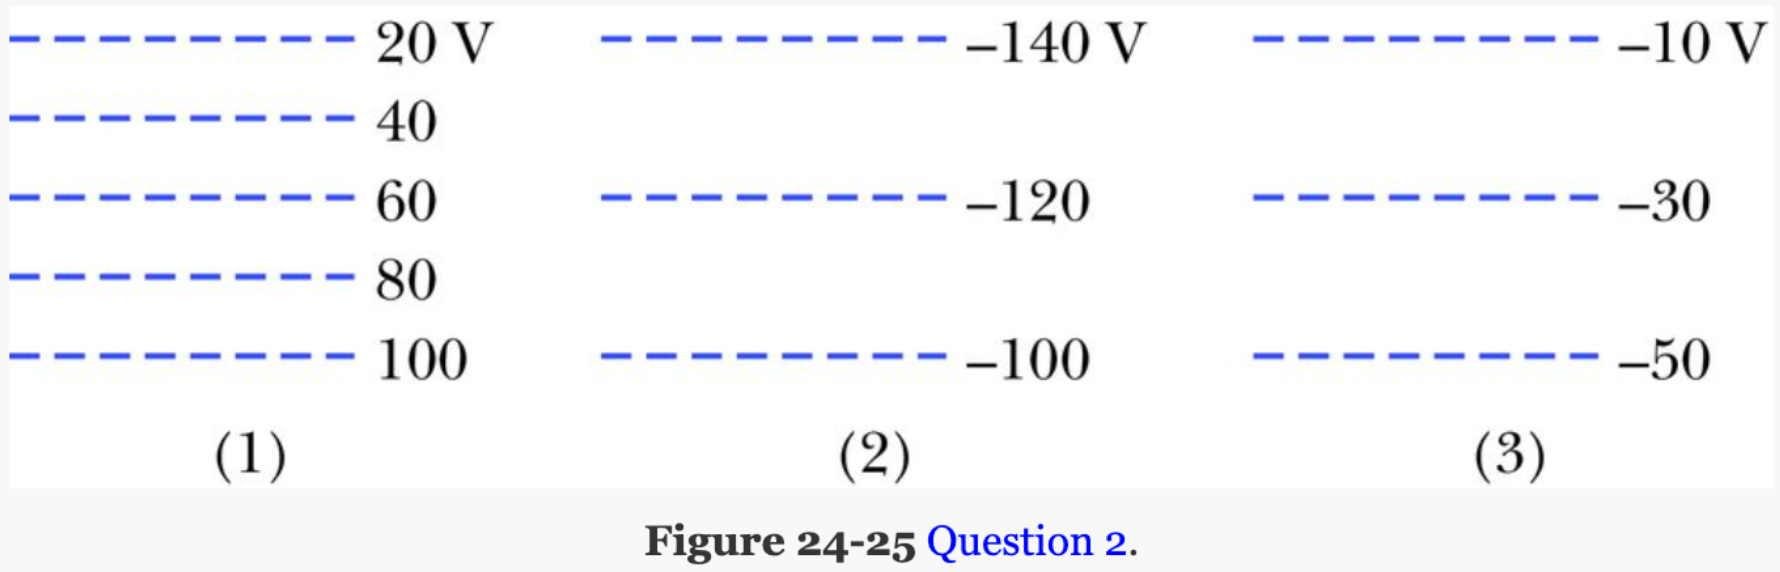
\includegraphics[width=\textwidth]{picture_1.png}

\subsection{Solution: (1) $>$ (2) = (3)}
We know that the formula for electric potential difference is proportional to the negative of th electric field, from the formula $\Delta V = -\int_i^f \vec{E}\cdot\,d\vec{s}$.
The inclusion of magnitude from the question means that direction does not matter, so we just have to rank $\Delta V$ from highest to lowest.
\begin{gather*}
    \left|\Delta V_1\right| = \left| 20 - 100 \right| = 80 \unit{\volt}\\
    \left|\Delta V_2\right| = \left| -140 - (-100) \right| = 40 \unit{\volt}\\
    \left|\Delta V_3\right| = \left| -10 - (-50) \right| = 40 \unit{\volt}
\end{gather*}
Thus, \boxed{V_1 > V_2 = V_3}.

\subsection{Solution: (3)}
Electric field lines point in the direction of lower electric potential.
The only case where electric potential is lower at the bottom than at the top is case (3).
As such, that is the only case where it is the case.
\pagebreak

\section{Question 3}
Figure 24-26 shows four pairs of charged particles. For each pair, let $V = 0$ at infinity and consider $V_{net}$ at points on the x axis. For which pairs is there a point at which $V_{net} = 0$ (a) between the particles and (b) to the right of the particles? (c) At such a point is $E_{net}$ due to the particles equal to zero? (d) For each pair, are there off-axis points (other than at infinity) where $V_{net} = 0$?
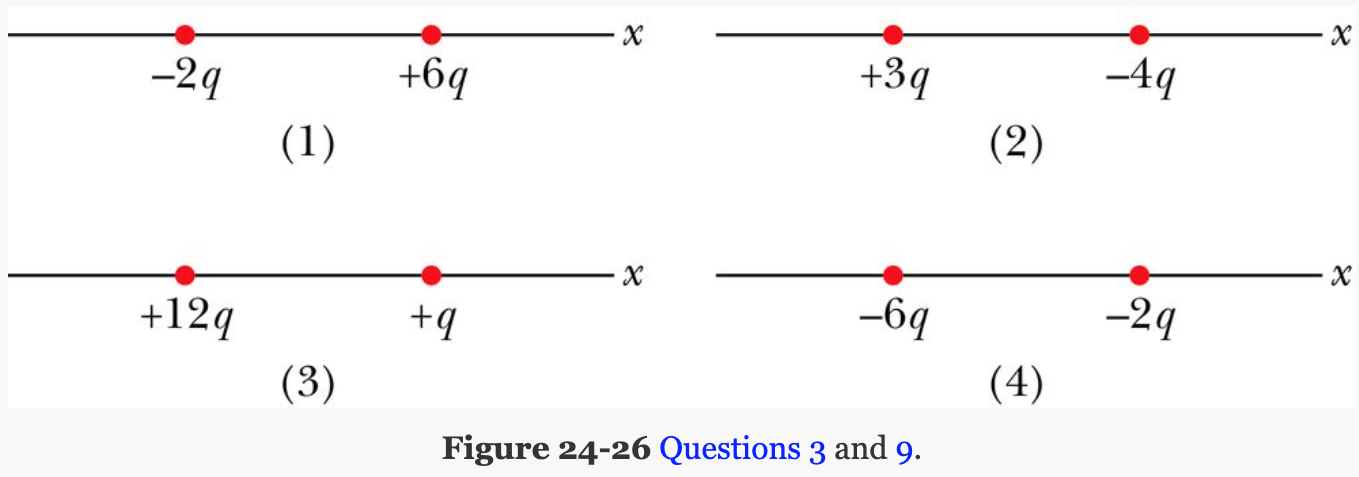
\includegraphics[width=\textwidth]{picture_2.png}

\subsection{Solution (a): 1 and 2}
For voltage, the formula is $V = \frac{kq}{r}$, and it has no direction. 
Thus, for each of the cases, since V has the same sign as q, we can know that there can only be a point at which the net voltage is zero when there is both a positive and a negative charge to influence the voltage.
The ratio of the magnitudes of the distances (radii) must also be the same as the ratio of the charges in order to make the sum equal to zero. 
\begin{gather*}
    0 = V_1 + V_2 = \frac{k\left|q_1\right|}{r_1} - \frac{k\left|q_2\right|}{r_2}\\
    \frac{k\left|q_1\right|}{r_1} = \frac{k\left|q_2\right|}{r_2}\\
    \frac{\left|q_1\right|}{\left|q_2\right|} = \frac{r_1}{r_2}
\end{gather*}
Between the two points, there must be a point at which the ratio holds true. 
This means that it holds true for \boxed{1 \text{ and } 2}

\subsection{Solution (b): None}
Since there is no point at which V = 0 on either (3) or (4), explained in part (a), we can rule them out. 
On both (1) and (2), the charge on the right is the stronger charge.
The aforementioned ratio will start with the ratio either too large or too small, and will keep heading away from an equal ratio ad infinitum as it heads further to the right. 
This leaves it with \underline{none}.

\subsection{Solution (c): No}
In these circumstances, there are no points to the right where V = 0 and only (1) and (2) have V = 0 between the two points. 
In the case of (1) and (2), between the two particles, the positive charge will be pushing the electric field away from itself, while the negative charge will assist this by frawing the electric field towards itself, increasing the magnitude of the electric field rather than decreasing it.
Having no points where the case is true, the answer is \underline{no}.

\subsection{Solution (d): Yes, so long as the charges have opposite sign.}
This is false for the electric field. 
However, because the electric potential is not a vector but a scalar, there will be a net zero electric potential anywhere that the formula from part (a) is true and the charges have opposite sign.
\pagebreak

\section{Question 9}
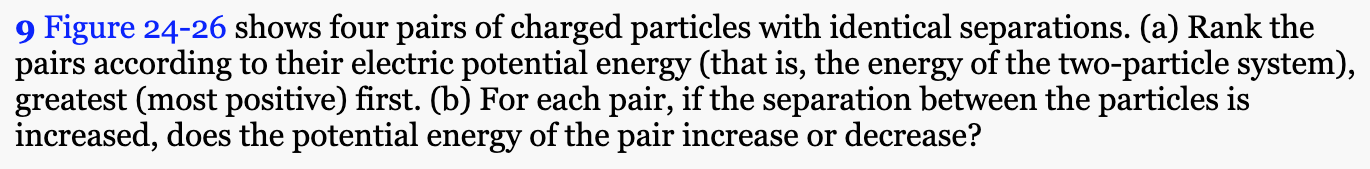
\includegraphics[width=\textwidth]{picture_3.png}

\subsection{Solution: (3) $>$ (1) $>$ (2) $>$ (4)}
We rank these by total charge in the system. 
(1) has total $4q$, (2) has total $-q$, (3) has total $13q$, and (4) has total $-8q$.

\subsection{Solution}
1) Decrease\\
2) Increase\\
3) Decrease\\
4) Increase
\pagebreak

\section{Question 11}
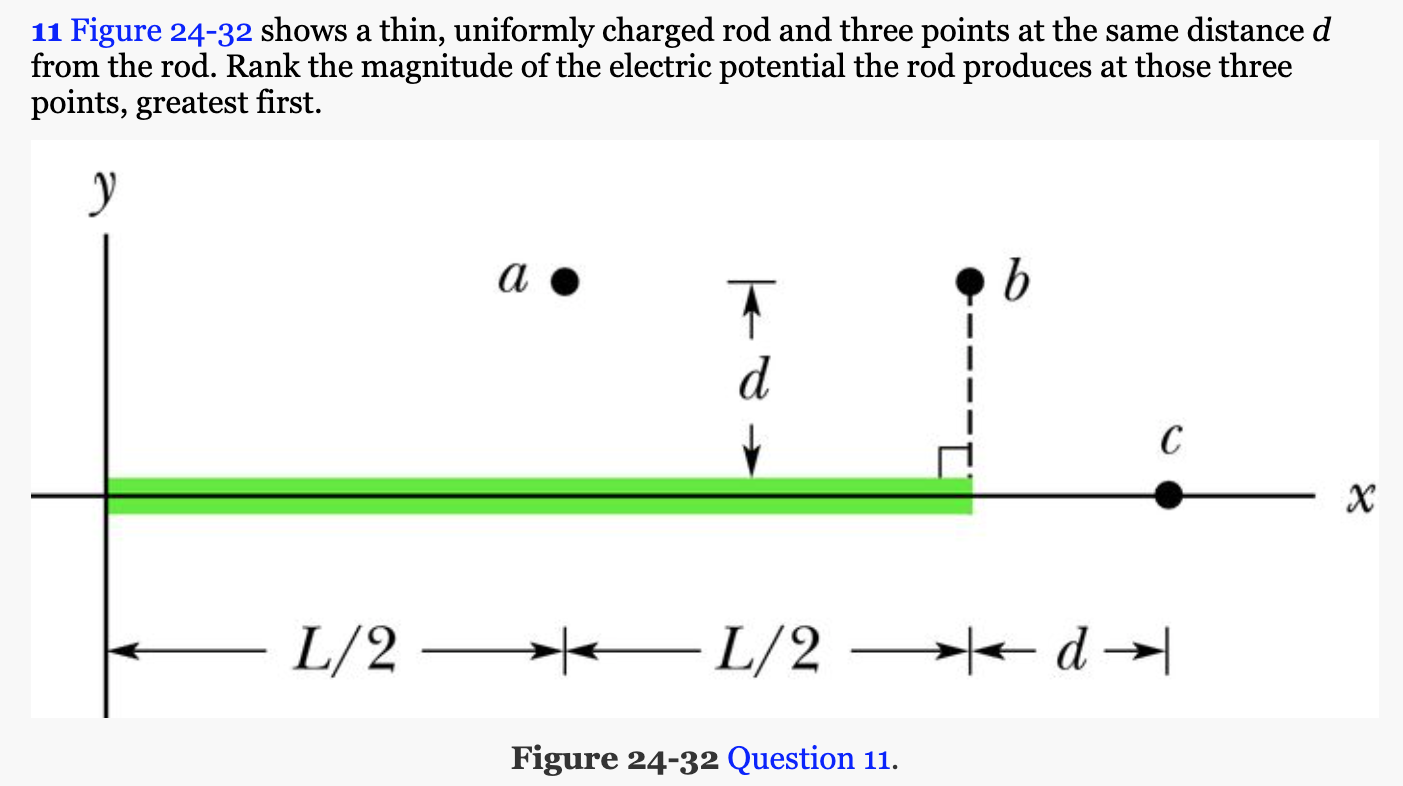
\includegraphics[width=\textwidth]{picture_4.png}

\subsection*{Solution: (a) $>$ (b) $>$ (c)}
There are an equal range through which electric potential is experienced for each point, but the distances have a different range.
I will be going through the points in my chosen order.\\
a) The range of distances ranges between $d$ and the pythagorean of $d$ and $L/2$, going through it twice over.\\
b) The range of distances is between $d$ and the pythagorean of $d$ and $L$. This being a larger range with a greater maximum value and the same minimum value, the total electrical potential would also be less. $(a) > (b)$.\\
c) The range of distances is between $d$ and $d + L$.  The triangle inequality tells us that the pythagorean between two sides of a triangle is less than the length of the two sides added together. As such, the distances will always be greater than in (b) for all points along the line charge. \boxed{(a) > (b) > (c)}.
\pagebreak

\section{Question 12}
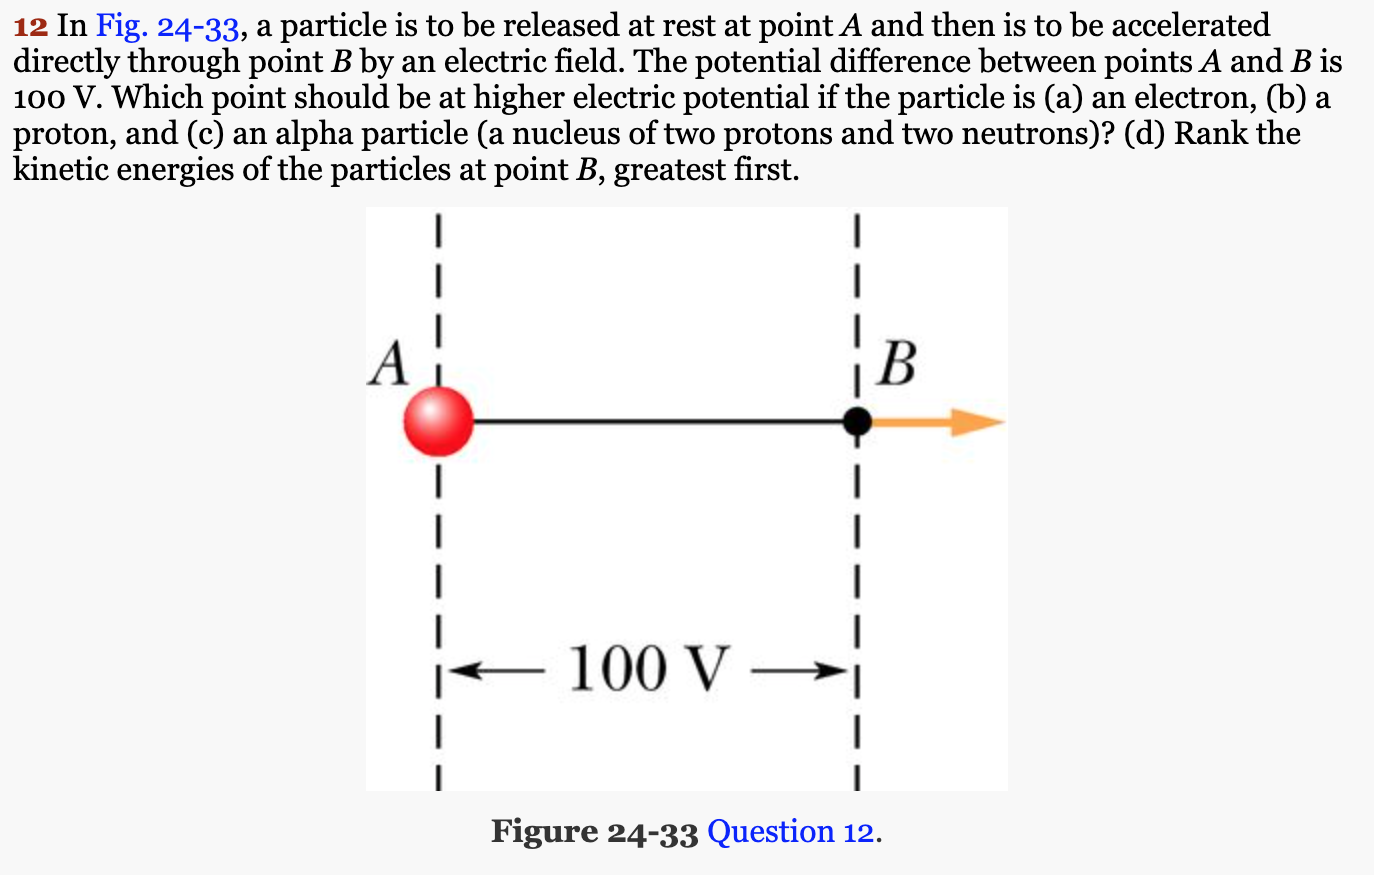
\includegraphics[width=\textwidth]{picture_5.png}

\subsection{Solution: B}
Electric field lines point in the direction of lower voltage (electric potential).
Negative charges go in the opposite direction as the electric field lines point.
Thus, negative charges go towards higher voltage if left alone.
As such, the end point must have higher electric potential, so the answer is \boxed{B}.

\subsection{Solution: A}
Positive charges go in the same direction as the electric field lines point.
Thus, positive charges go towards lower voltage if left alone.
As such, the end point must have lower electric potential, so the answer is \boxed{A}.

\subsection{Solution: A}
An alpha particle contains only positive charge (2 protons). 
As such, it will behave like any other positively charged particle would, so the answer is \boxed{A}.

\subsection{Solution: Alpha particle $>$ Proton = Electron}
We know that $\Delta K = -q \Delta V$.\\
\underline{Electron}: The electron has negative charge, but the change in voltage will be positive.
As such, the electric potential difference would be a negative multiplied by a negative, so positive, with a value of $100*e$.\\
\underline{Proton}: The proton has positive charge, but the change in voltage will be negative (previously established).
As such, the electric potential difference would be a negative multiplied by a negative, so positive, with a value of $100*e$.
Proton = Electron.\\
\underline{Alpha particle}: The alpha particle has positive charge equal to twice that of a proton ($2e$), but the change in voltage, as previously established, will be negative.
As such, the electric potential difference will be a negative multiplied by a negative, so positive, with a value of $200*e$.
\boxed{\text{Alpha particle $>$ Proton = Electron}}
\pagebreak

\section{Problem 6}
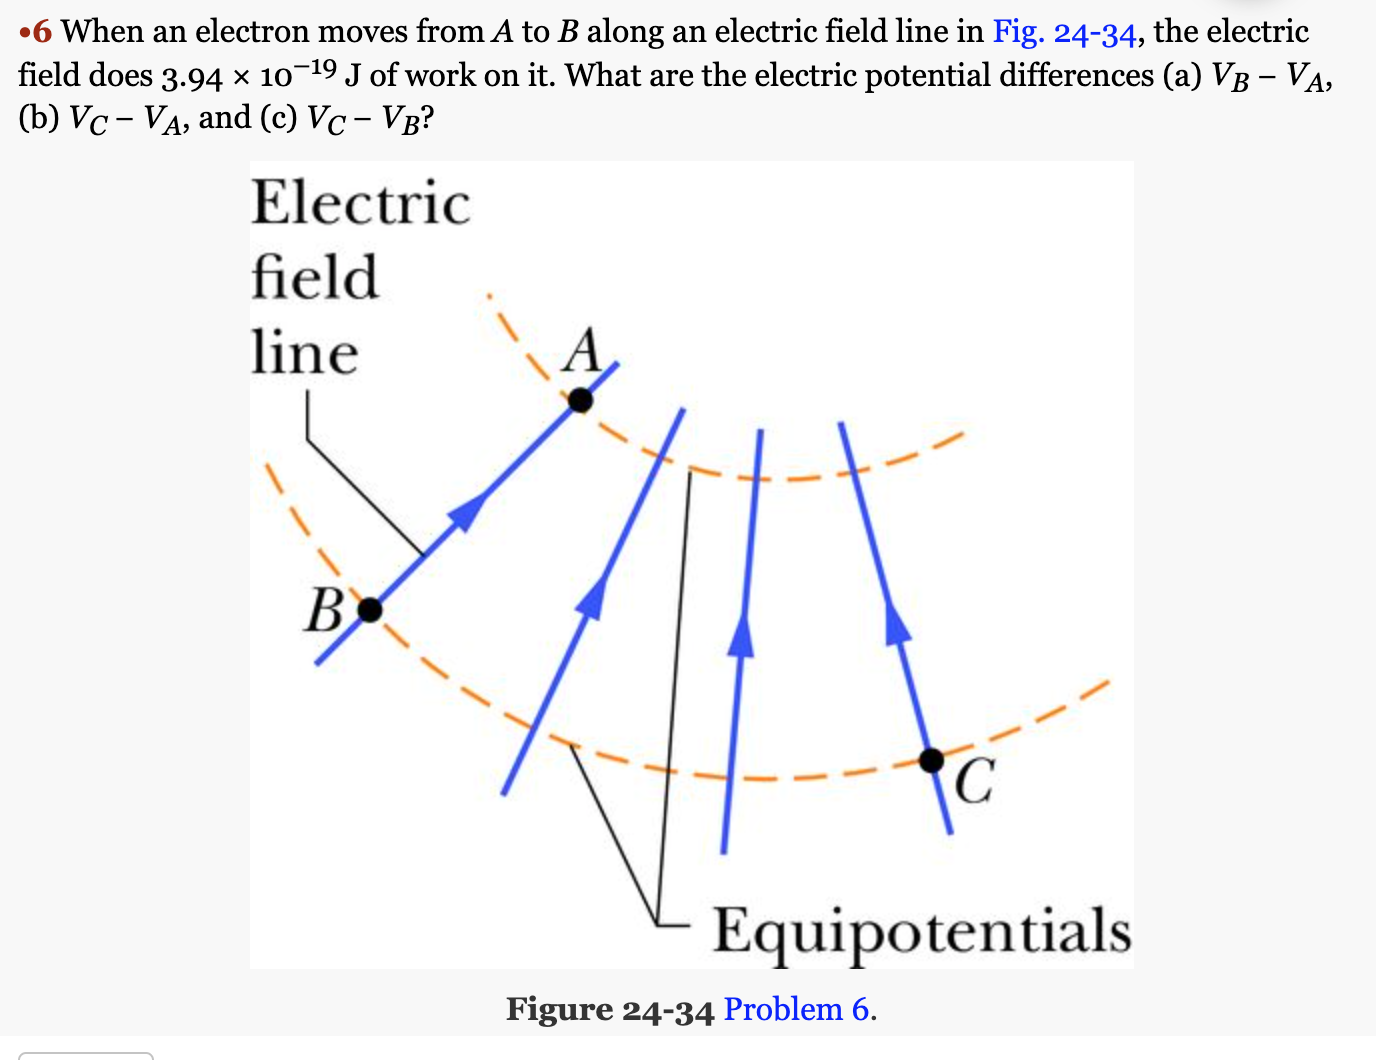
\includegraphics[width=\textwidth]{picture_6.png}

\subsection{Solution: 2.46V}
We know the formula for work done on an object and how that relates to the electrical potential difference.
We can use what we know to get what we need.
\begin{align*}
    W_{app} &=  q\ \Delta V\\
    \Delta V    &=  \frac{W_{app}}{q}
        =   \frac{3.94 \times 10^{-19} \unit{\joule}}{1.602 \times 10^{-19} \unit{\coulomb}}
        =   \frac{3.94}{1.602} \unit{\joule/\coulomb}
        =   \boxed{2.46 \unit{\volt}}
\end{align*}

\subsection{Solution: 2.46V}
Due to path independence, it would be equal to going across the equipotential line to point B from point C (along which $\Delta V = 0$), then following the same path as before to get to point A.
It would have the same value as that between points B and A.

\subsection{Solution: 0}
The two points lie along the same equipotential line. 
Along equipotential lines, the electric potential remains constant.
As such, between the two points, the difference is \boxed{zero}.
\pagebreak

\section{Problem 8}
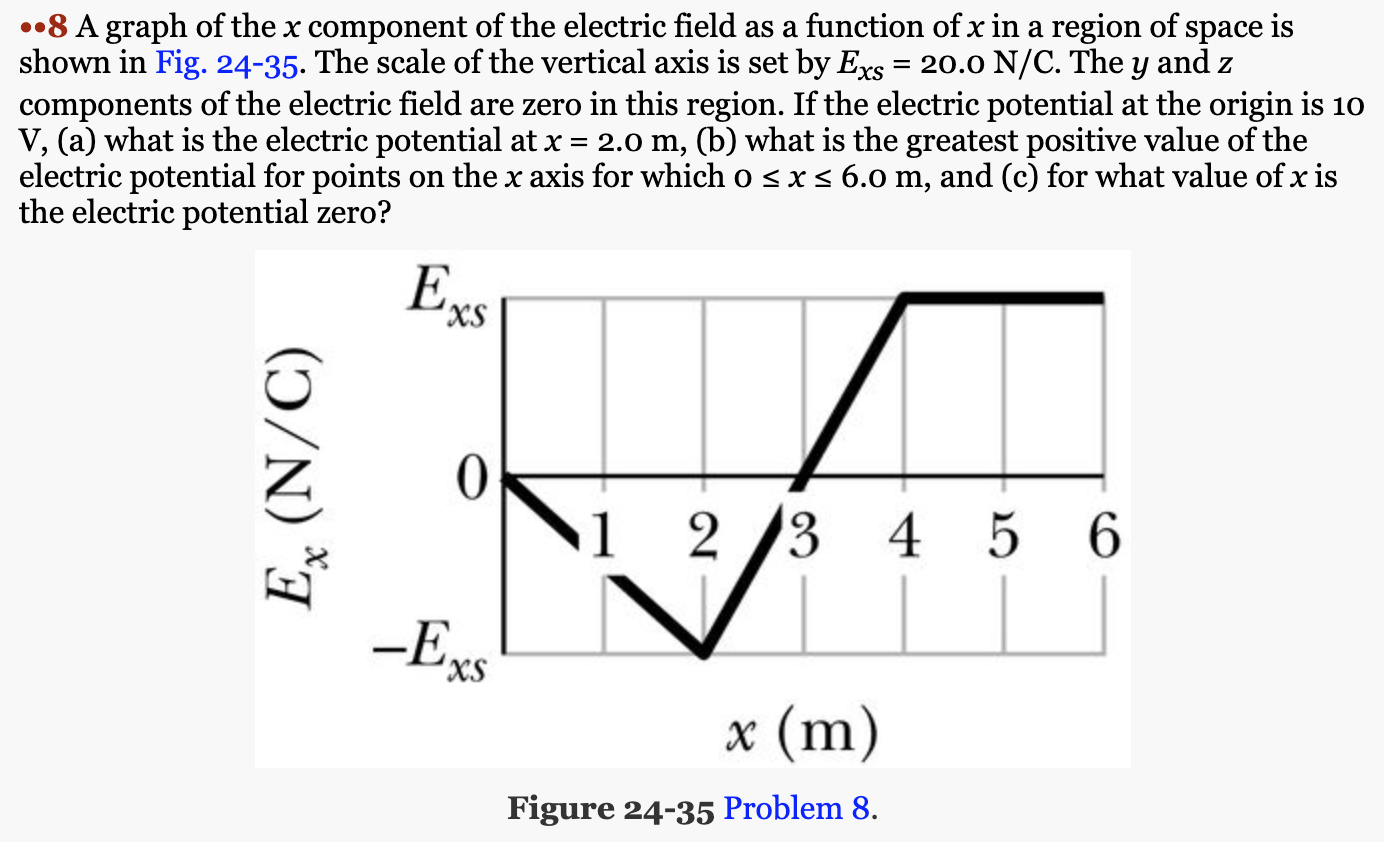
\includegraphics[width=\textwidth]{picture_7.png}

\subsection{Solution: 30V}
We can define the function. 
\(E(x) = \left\{ \begin{matrix}
    0 \le x < 2| \\
    2 \le x < 4| \\
    4 \le x < 6| 
\end{matrix}
\begin{matrix}
    \frac{-20}{2}x\\
    \frac{40}{2} - 60\\
    20
\end{matrix} \right\}\)
We will only be working with one dimension.
\begin{align*}
    \Delta V &= -\int_{0}^{2} E(x)\,dx
        =   \int_0^2 10x\,dx
        =   \left. 5x^2 \right|_0^2
        =   20 + 0
        =   20 \unit{\volt}\\
    V_f &=  V_i + \Delta V
        =   10 \unit{\volt} + 20 \unit{\volt}
        =   \boxed{30 \unit{\volt}}
\end{align*}

\subsection{Solution: 40V}
Since the electric field is the negative derivative of the electric potential difference, the point at which the electric potential difference would be maximum would be where the electric field would be zero crossing from negative into positive. 
Aside from the origin, the only spot where this is the case is at x = 3.
\begin{align*}
    \Delta V &= -\int_{0}^{3} E(x)\,dx\\
        &=  -\int_{0}^{2} E(x)\,dx - \int_{2}^{3} E(x)\,dx\\
        &=  \int_{0}^{2} 10x\,dx - \int_{2}^{3} 20x - 60\,dx\\
        &=  \left. 5x^2 \right|_0^2 - \left[ 10x^2 - 60x \right]_2^3\\
        &=  20 \unit{\volt} - (90 - 40 - 60) \unit{\volt}\\
        &=  20 + 10 \unit{\volt}
        =   30 \unit{\volt}\\
        V_f &=  V_i + \Delta V
        =   10 \unit{\volt} + 30 \unit{\volt}
        =   \boxed{40 \unit{\volt}}
\end{align*}

\subsection{Solution: x=5.5m}
From x=0 to x=2, the electric potential increases until $V = 30\unit\volt$. 
Between x=2 and x=4, the voltage increases, then decreases, canceling itself out. 
Due to properties of integration, we can find the value of x for whch $20(x - 4) = 30$. 
The value for which that is the case, or the solution is x=5.5.
Adding units, we get \boxed{x = 5.5\unit{\meter}}.  
\pagebreak

\section{Problem 10}
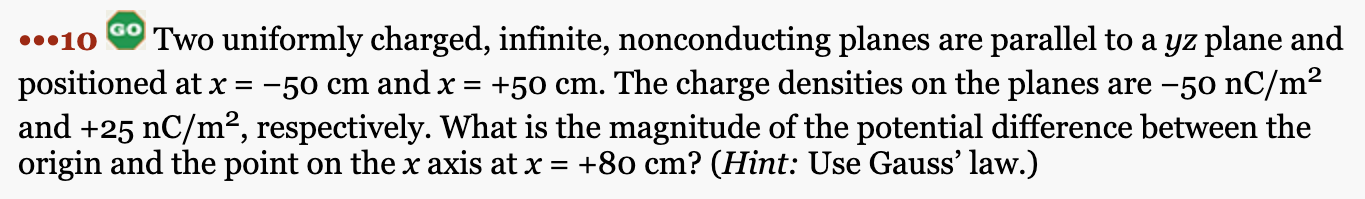
\includegraphics[width=\textwidth]{picture_8.png}

\subsection*{Solution}
By Gauss' Law, we know that the electric field from an infinite nonconucting plate is equal to $E = \frac{\sigma}{2\varepsilon_0}$.
The electric potential is equal to the integral $\Delta V = \int_{i}^{f} \vec{E}\cdot d\vec{s}$.
We can separate that integral into two halves, one between the orgin and the top plate, and the other between the top plate and x = 80cm.
From that, we can compute the electric fields and subsequently the voltage.
We can label the plate at x = 50cm to be plate 1 and the plate at x = -50cm to be plate 2.
The vectors of the electric field and the motion are in the same direction, so we can just replace the dot product with multiplication.
Check it out.
\begin{align*}
    \Delta V    &=  \int_{0\unit{\meter}}^{0.8\unit{\meter}} \vec{E} \cdot d\vec{s}
        =   \int_{0.5\unit{\meter}}^{0.8\unit{\meter}} \vec{E} \cdot d\vec{s} + \int_{0\unit{\meter}}^{0.5\unit{\meter}} \vec{E} \cdot d\vec{s}\\
        &=  \int_{0.5\unit{\meter}}^{0.8\unit{\meter}} E \,ds + \int_{0\unit{\meter}}^{0.5\unit{\meter}} E \,ds\\
        &=  (E_1 + E_2) \int_{0.5\unit{\meter}}^{0.8\unit{\meter}} \,ds + (E_1 - E_2) \int_{0\unit{\meter}}^{0.5\unit{\meter}} \,ds\\
        &=  (E_1 + E_2)*0.3 + (E_1 - E_2)*0.5\\
        &=  \left(\frac{\sigma_1}{2\varepsilon_0} + \frac{\sigma_2}{2\varepsilon_0}\right)*0.3 + \left(\frac{\sigma_1}{2\varepsilon_0} - \frac{\sigma_2}{2\varepsilon_0}\right)*0.5\\
        &=  0.8*\frac{\sigma_1}{2\varepsilon_0} - 0.2*\frac{\sigma_2}{2\varepsilon_0}
        =   \frac{0.4*\sigma_1 - 0.1*\sigma_2}{2\varepsilon_0}\\
        &=  \frac{0.4*(-50 \times 10^{-9}) - 0.1*(25 \times 10^{-9})}{2*(8.85 \times 10^{-12})}\\
        &=  \frac{-20 - 2.5}{17.7} \times \frac{10^{-9}}{10^{-12}}
        =   -\frac{17.5}{17.7} \times 10^3
        =   -998.7 \unit{\joule/\coulomb}\\
    \left|\Delta V\right|   &=  \left|-998.7 \unit{\joule/\coulomb}\right|
        =   \boxed{998.7 \unit{\joule/\coulomb}}
\end{align*}
\pagebreak

\section{Problem 16}
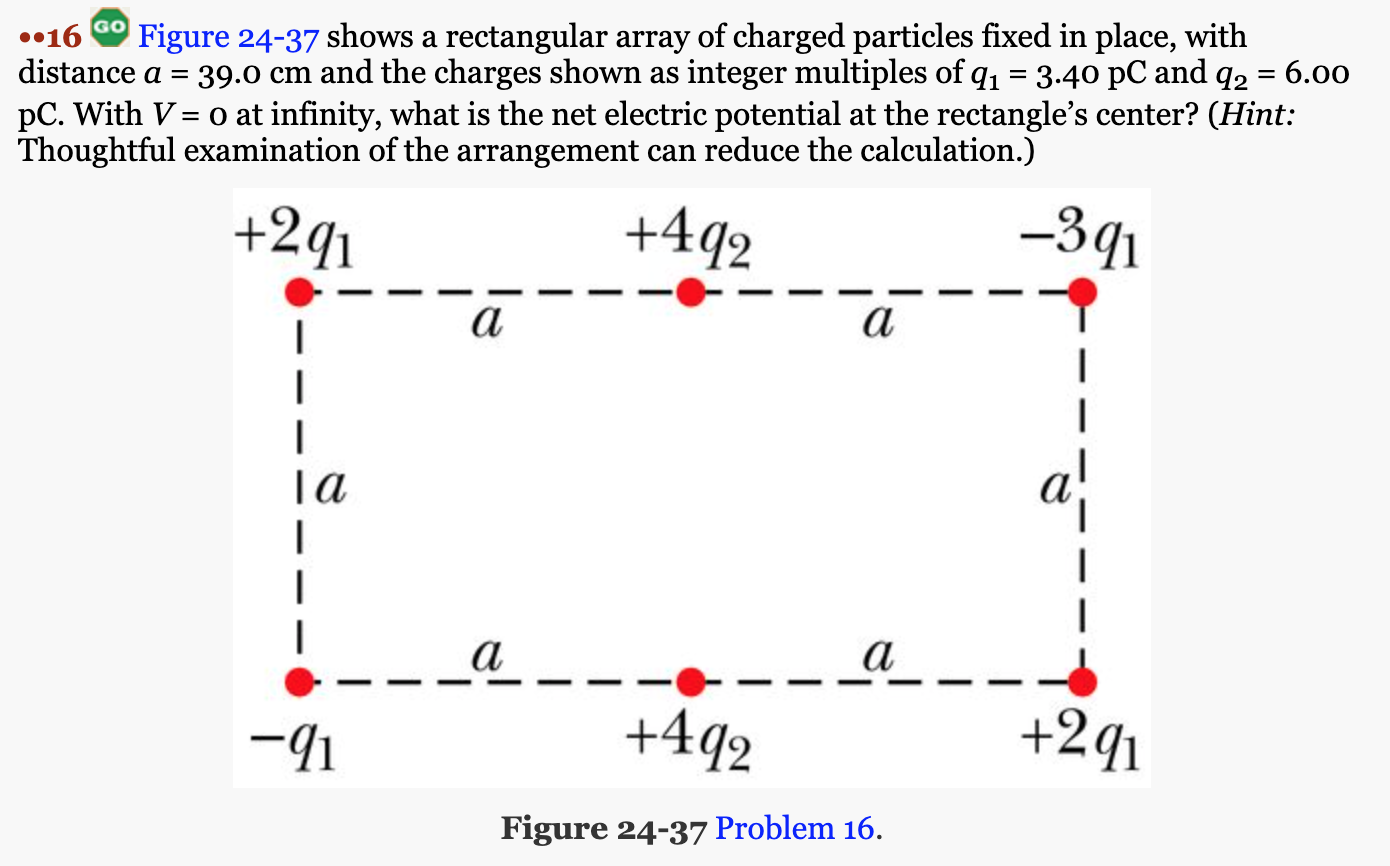
\includegraphics[width=\textwidth]{picture_9.png}

\subsection*{Solution: 2.214 \unit{\joule/\coulomb}}
Let's start with the corners.
Suppose the distance between the corners and the center is a distance $r_1$. Each of them is multiplied by $q_1$.
We can form a formula for the electric potential due to the four corners.
\begin{align*}
    V_{corners} &=  V_{11} + V_{12} + V_{21} + V_{22}\\
        &=  \frac{k*2q_1}{r_1} + \frac{k*(-3q_1)}{r_1} + \frac{k*(-q_1)}{r_1} + \frac{k*2q_1}{r_1}\\
        &=  \frac{kq_1}{r_1}(2 - 3 - 1 + 2)
        =   \frac{kq_1}{r_1}(4 - 4)
        =   \frac{kq_1}{r_1} * 0
        =   0
\end{align*}

Thus, we only need concern ourselves with the charges on the sides, each of which are only $\frac{a}{2}$ away from the center.
We can use a like formula for the two.
\begin{align*}
    V_{sides}   &=  V_{top} + V_{bottom}
        =   \frac{k*4q_2}{\frac{a}{2}} + \frac{k*4q_2}{\frac{a}{2}}\\
        &=  \frac{2*k*4q_2}{a} + \frac{2*k*4q_2}{a}
        =   \frac{16kq_2}{a}\\
        &=  \frac{16 * (8.99 \times 10^9) * (6.0 \times 10^{-12})}{39 \times 10^{-2}}\\
        &=  \frac{(143.84 \times 10^9) * (6.0 \times 10^{-12})}{39 \times 10^{-2}}\\
        &=  \frac{863.04 \times 10^{-3}}{39 \times 10^{-2}}
        =   \boxed{2.214 \unit{\joule/\coulomb}}
\end{align*}
\pagebreak

\section{Problem 30}
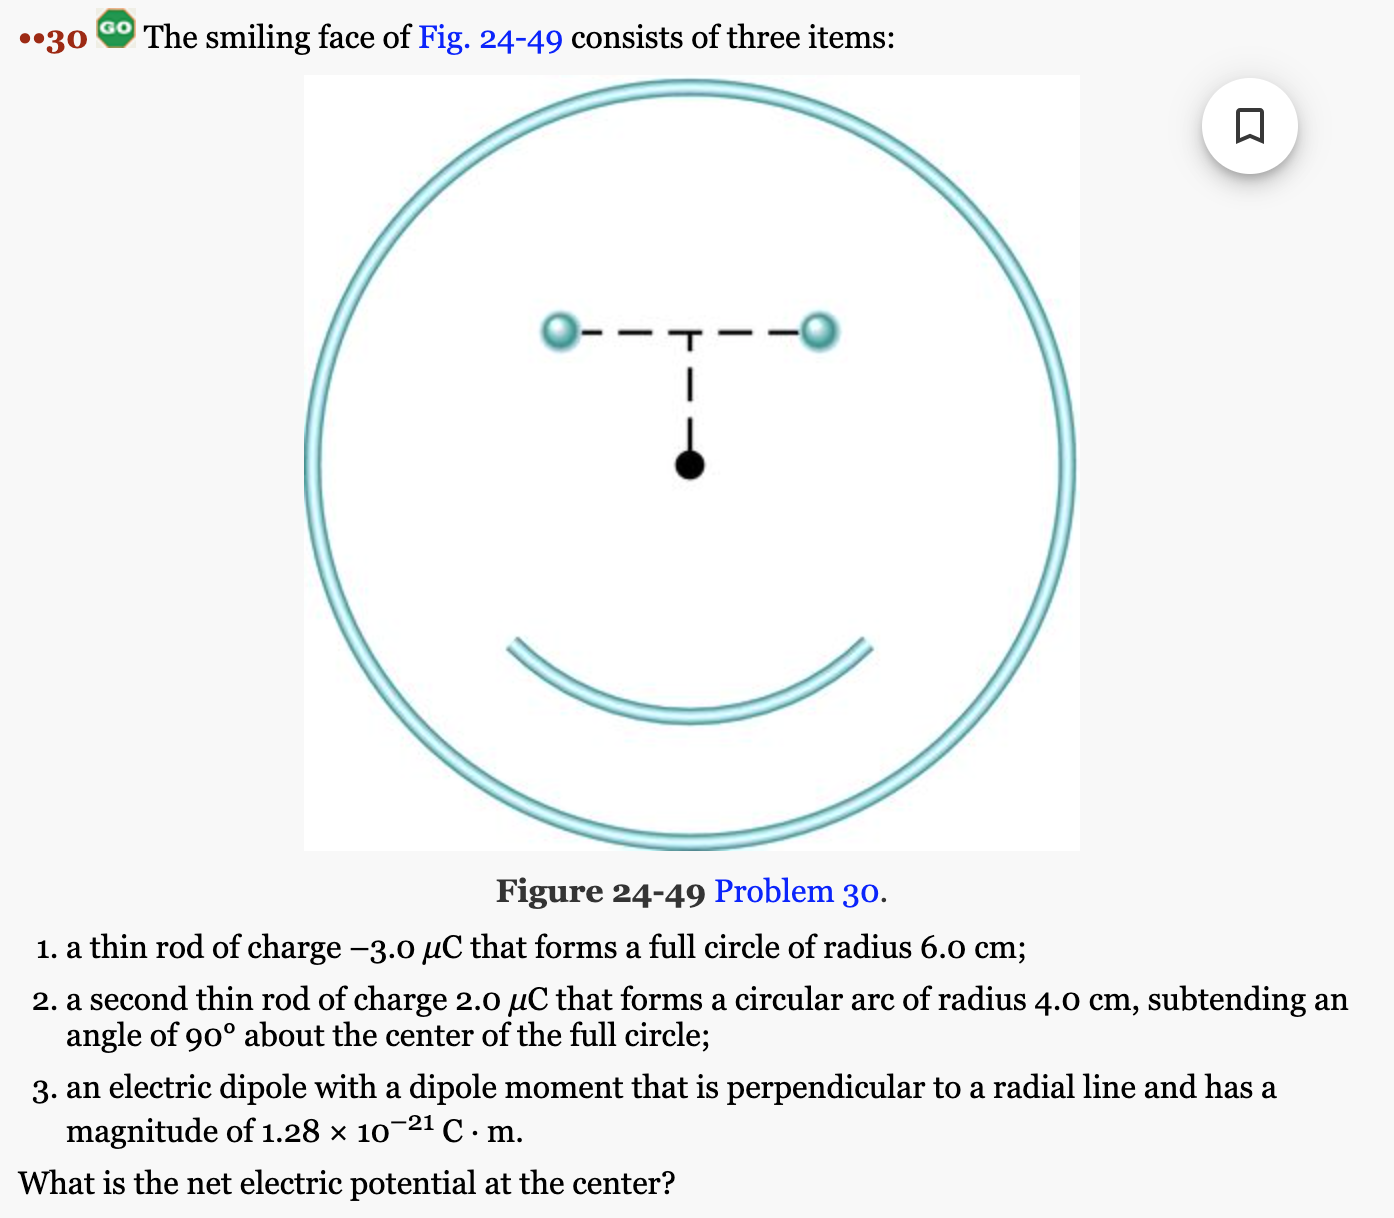
\includegraphics[width=\textwidth]{picture_10.png}

\subsection*{Solution: 0V}
Electric potential has no vectorial direction. 
For this problem, in order to make things easier, I will start by 
% proving 
saying that the electrical potential from a line charge where all points on it are the same distance from the point is the same as the electric potential if the whole charge were concentrated in one place the same distance from the point.
We can apply that to both the thin rods, calculating the voltage for both.
Additionally, for the dipole, the charge is equal and opposite for both particles, as is the distance between the two, making the two cancel out each other since electric potential has no vectorial direction.
\begin{align*}
    V_{net} &=  V_1 + V_2
        =   \frac{kq_1}{r_1} + \frac{kq_2}{r_2}
        =   k\left(\frac{-3 \times 10^{-6}}{6 \times 10^{-2}} + \frac{2 \times 10^{-6}}{4 \times 10^{-2}}\right)\\
        &=  k\left( -\frac{1}{2} + \frac{1}{2} \right) \times 10^{-4}
        =   k * 0 \times 10^{-4} \unit{\joule/\coulomb}
        =   \boxed{0 \unit{\volt}}
\end{align*}

\end{document}